%This is a narrative description of the general context within which your project fits. Depending on your particular project characteristics, you are required to include discussion of any or all of the following – previous related work; the work or objectives of a client; the essential principles of systems or techniques you are using.%

%All this narrative should be properly referenced to source material citations. Remember that a high class project will refer to background sources beyond just those on the Web. %

%In writing this section you should pay close attention to your audience and their prior knowledge of the subject(s) that you are discussing. You should assume that your reader is a student who has just completed the second year of your degree programme and can therefore assume that the reader is familiar with all topics taught up to the end of the second year. Anything that is needed to understand your project and its context but which has not been taught by the end of the second year of your degree should be discussed in this background section. %

%This section may include one or more of the following subsections. It is difficult to give prescriptive guidance on which subsections you should include as this depends on the nature of the project you are undertaking – you should discuss this with your supervisor.%
\chapter{Background}

%Problem Context:
%If your project involves significant work on a non-computing topic that is likely to be unfamiliar to most readers (e.g. linguistics, fluid dynamics) you should describe the important principles, concepts and terminology of that subject area in some detail. You will have had to learn these yourself in getting to grips with this unfamiliar topic and you should summarize what you learnt to enable the reader to understand your subsequent discussion on your project work and how this relates to the wider topic area.
\section{Problem Context}

The main focus of this project is to create a network degradation tool that can be used to simulate imperfect network conditions and common attacks. To understand the goal better it is important to know which criteria reduce network quality.

Latency, packet loss and bandwidth are the main factors that distinguish between good and bad internet connections. Latency is the delay between sending a message and seeing its result. Packet loss is the percentage of packets that are lost in a transmission, the higher the percentage, the more effect it has on the speed and stability of the network. Bandwidth is the measure of how many bits/bytes are being transferred per second, the larger the bandwidth the more data can be transferred in less time, thus making the overall connection faster. A combination of favourable values from these criteria defines a good network connection. One way to visualise the throughput of a network connection is a download and upload speed test. The result of these test are measured in Mbps and can be used to quickly compare the speed of two connections.

Other small signs of poor network conditions are Jitter and Error rate. Jitter is simply the variance in inter packet gaps (time gap between two packets). The gap is normally an issue that exists in large packet switched networks. TCP based communications are not normally affected heavily by jitter due to the way that the TCP protocol deals with these issues. However, the UDP based VoIP (Voice over IP) protocol is visibly degraded by heavy jitter. Error rate is the number of bit errors that have occurred in a data stream over a period of time. This can again effect UDP based communications heavily but the TCP protocol mitigates the effects and therefore remains relatively unaffected.

It is also necessary to mention in more detail the protocols that are to be used in the network simulation section. TCP \citep{TCP} and UDP \citep{UDP} are the transport layer protocols up for discussion. 

\clearpage
\subsection{Protocols}
\subsubsection{Transport Control Protocol (TCP)}
TCP's main design choices are centred around reliability, where it has a few techniques designed to make sure packets arrive correctly. 


\begin{center}
	\includegraphics[scale=0.7]{TCP_header}
	\begin{figure}[h]
		\caption{TCP Header (RFC 793)}
	\end{figure}	
\end{center}

\subsubsection*{Initiating a connection}
The connection is initiated with a series of signals carried as packets. These signals are abbreviated as ACK (Acknowledgement) and SYN (Synchronise). The initiating party begins by sending an empty packet with the SYN flag set, this starts the synchronization process. Then once the target computer receives this SYN packet it sends back an ACK plus its own SYN packet (This is normally sent as a single ACK + SYN packet). Where finally the initial computer sends back an ACK packet in response to the previous SYN packet, this connection has now been initiated and the communication channel has been set up. This process is known as a `3-way handshake'.

\begin{center}
	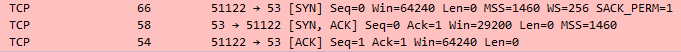
\includegraphics[scale=0.8]{SYN-ACK}
	\begin{figure}[h]
		\caption{The output from Wireshark showing the handshake}
	\end{figure}
\end{center}

\clearpage
\subsubsection*{Sequence Numbers and Acknowledgement Numbers}
One of the main mechanisms for detecting missing and incorrect packets is the sequence and acknowledgement numbers. The sequence number is increased by the length of every correctly transmitted packet. A packet's length can be calculated by taking the total size of the packet and subtracting the size of the header. For example, if a packet with a length of 100 was sent it would move the sequence value up by 100, this gives the protocol the information to judge what it should be expecting and what it has received. If these values do not add up, TCP can flag for an error and retransmit.

To guarantee arrival of a packet the sender needs to know when packets have been received, this is where the acknowledgement number comes in. Packets carrying acknowledgements are known as ``ACKs". For a packet with a sequence number of 100 being sent, it will require a packet to be returned containing the ACK number of 100 to verify that exact packet has been transferred correctly. If the corresponding ACK packet is not received before the time-out value has been reached the packet is resent, this is how TCP guarantees retransmission of packets. TCP's guaranteed arrival is one of the reasons why packet loss does not have the same devastating effect it does on UDP with TCP.

In situations where connections are created and recreated quickly in succession or are being quickly re-established after errors there cannot be initial sequence numbers (ISN) that clash with previous segment that may still exist on a network connection. Therefore TCP solves this issue by generating new ISNs using a ISN Generator that uses a 32 bit clock. The 32 bit clock has a life cycle of 4.55 hours where this time period is commonly known as the Maximum Segment Lifetime (MSL). If an ISN is generated within this MSL, it can be guaranteed to be unique.

\subsubsection*{Receiving Window}
In the TCP header there is a two byte value that represents the receiving window size, this value defines the maximum size of unacknowledged packets the receiving end has space for. If a client sends a packet with a 65535 window size value it tells the receiving computer not to send more than 65535 bytes before receiving corresponding acknowledgements. This value can also be extended using a value in the area allocated in the `TCP Options' called `Window Scaling', this allows the value in the window size to be multiplied by this scale value. For example, a window size of 65535 with a window scale of 5 would have a total window size of 327675 Bytes. A larger window size means more data can be sent before the protocol needs to wait for acknowledgements and can normally mean faster transfer speeds. It is worth noting; this exchange of window scaling values is only performed in the handshake and can only be present in the initial exchange of packets.

\subsubsection*{Flow Control}
Flow control is a mechanism used by the protocol to ensure that the receiving party does not become overwhelmed by the incoming transmission of packets. TCP has two types of buffers the `send' and `receive', where the send buffer collects what data is going out and the receive buffer collects what is coming in. The purpose of the flow control is to prevent the sending of packets that will not fit in the destination receive buffer and therefore will prevent these packets from being dropped. The protocol achieves this by allowing each party to advertise its available receive buffer space through the `Window Size' section in the header (This is included in each ACK packet) and is commonly known as the `Advertised Window`. Once the receive buffer is full the receiving party will advertise what is known as a `zero window' where it sets the window size to zero and transfer will halt until there is adequate space in the receive buffer.

\subsubsection*{Sliding Window}
\label{ref:window}
To control the number of packets the protocol has in flight at any one time the protocol utilises the `sliding' window. The size of the sliding window is altered by two factors: The size of the send buffer and the size of the destinations receive buffer. Therefore, the maximum amount of data the protocol can send is the smallest of the two previous values. 
\begin{center}
	$SlidingWindowSize = Min(LocalSendBuffer, DestinationRecieveBuffer)$
\end{center}
The sliding window then dynamically works out how many packets it can send by keeping track of the number of packets in flight (unacknowledged) and the amount left of the current window size. This whole process gives the protocol the ability to dynamically adapt to changing conditions and aims to prevent buffers from being overfilled.


\subsubsection*{Closing a connection}
The closing of a TCP connection is very similar to the initial construction \citep{TCP}, but in this case the protocol utilises the `FIN' flag defined in the TCP header. In this example it will be a client disconnection from a server. After all the data is transferred the client no longer requires a connection to the server and sends an empty packet with the FIN bit set, the server receives the packet and returns an ACK. The server now sends its own FIN and this is then acknowledged by the client. This middle step with the server sending an ACK and FIN separately is normally performed in a single packet in live networks. The client and server now knows the connection is closed and will free up any resources allocated to that connection.



\subsubsection*{Congestion control}
\label{ref:tcpCongestion}
In situations where multiple clients are connected to a single receiver, the bandwidth needs to be split equally between the clients. This is performed by the inbuilt TCP congestion control. The clients send data and keep increasing their transfer rate until they loose a packet. Packet loss is therefore a sign of congestion - this is because it assumes that the packets are being lost due to the router having insufficient packet buffering space. When the number of clients drops, more bandwidth then becomes available and the congestion algorithm utilises this naturally because it has been periodically probing the network to check for available bandwidth. This probing is done by increasing its transfer rate until packet loss is encountered, where it then quickly slows its transfer rate and repeats the process. This results in TCP auto balancing when new clients are introduced and removed and thus utilizing as much bandwidth as is available.

The rate of transfer is indirectly defined by two values "Congestion Window" (Cwnd) and "Advertised Window". The congestion window is the amount of packets a connection stream allows in flight and the advertised window is used to inform the sending end how much buffer space is available to hold incoming packets. These both define the overall "WinSize" where a small value means fewer packets can be sent without waiting for corresponding acknowledgements and therefore reducing the transfer speed. The equation below is used to define window size: 

\begin{center}
	$WinSize = Min(CongestionWindow, AdvertisedWindow)$
\end{center}

Later this report will discuss the effects of packet loss, latency and other degradation signs on this congestion control.

 
\subsubsection*{AIMD}
AIMD, standing for Additive Increase Multiplicative Decline, is a feedback control algorithm known for its use in TCP's congestion control. It works by having a linear increase and exponential decline and it will naturally mean that if set up correctly all entities using AIMD will converge on equal usage of a shared resource - in this case network bandwidth. This famously produces a 'saw-tooth' pattern when the maximum capacity is reached \citep{huston2006gigabit}.

\subsubsection*{Slow Start}
\label{ref:slowstart}
Slow start is designed for defining suitable initial transfer rates of a TCP connection. The slow start mechanism is required because an initial huge transfer rate will have a high chance to cause the receiving buffer to overflow and will revert the connection to a crawl. Therefore, the solution to this is to start with a small-medium transfer rate and increase it per acknowledgement received.

\subsubsection*{Congestion Algorithms}
There are various algorithms used to manage congestion on a network and they work in slightly different ways. All algorithms have situations where they work most effectively.


\subsubsection*{Congestion Algorithm - TCP Reno}
TCP Reno was first released in the 4.3BSD OS and is normally grouped up with TCP Tahoe as they share many features. TCP Reno uses AIMD  where it performs its additive increase when a full window is transferred correctly and its multiplicative decline when a packet is lost. It introduces two new ideas "Fast Retransmit" and "Fast Recovery":

{\it Fast Retransmit}\\
This mechanism uses 3 duplicated acknowledgements (these can be caused by re-ordered or missing segments) to signal the need for a retransmission. Fast Retransmit can repair single segment loss and does not involve the use of any time-outs, this lack of time-outs can involve a lot less idle link time. After this the congestion window size is reduced by half because of detection of loss.

{\it Fast Recovery}\\
For every duplicate ACK a segment must arrive, this can therefore be used to assume that the receiving of a segment means the buffer in the receiving end has more space available. Therefore, the sending of more packets has a low chance to cause the buffer on the receiving end to overflow - thus, new segments are put onto the network when any acknowledgements are received (even duplicated acknowledgements). 

These techniques are both used together and can result in effective mitigation of packet loss.

Reno defines congestion problems in terms of packet loss and can be defined either of two ways:

\begin{itemize}
	\item Three duplicated acknowledgements are considered non-severe and the algorithm moves into congestion avoidance with Fast Retransmission and Fast Recovery coming into effect.
	\item Retransmission defined by a time out is defined as {\bf severe} and will set the Congestion Window to the minimum value and initiate a Slow Start. Time outs are usually caused by multiple occurrences of packet loss.
\end{itemize}

\subsubsection*{TCP NewReno}
NewReno \citep{newReno} as the name suggests is the successor to TCP Reno that was discussed in the previous section. It is the version of Reno used in recent versions of the Linux Kernel.

TCP NewReno uses further heuristics to recover from multiple packet loss without the need for time-outs. This therefore means it outperforms Reno at higher error rates and is the algorithm used in the later experimentation section of this report.

\subsubsection{User Data Protocol (UDP)}
\begin{center}
	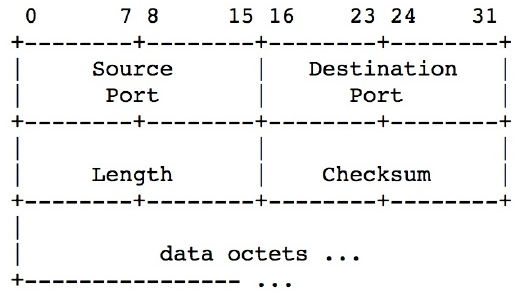
\includegraphics[scale=0.7]{udp_header}
	\begin{figure}[h]
		\caption{UDP Header (RFC 768)}
	\end{figure}		
\end{center}

UDP is by design the opposite of TCP and often you'll find the two protocols compared. UDP is often referred to as ``fire and forget" \citep{kempf2011thoughts} this is a short way of describing how UDP deals with packets. Once a packet is sent UDP then and moves onto the next. However, this means aside from the checksum in the UDP header (which can be used to check that the UDP data has been transferred correctly) there is no error checking for the UDP protocol, resulting in UDP being considered unreliable in comparison to TCP. 

The absence of error-checking overhead, however, greatly improves the speed of UDP protocols. UDP is not used in situations where communication is vital, but does find itself implemented in examples like voice or video chat because errors in these services are not catastrophic to operation and these imperfections can even go unnoticed.

As the very small UDP header shows, it is a very simple protocol and is effectively a thin wrapper on top of the IP layer. UDP allows for very quick transfers but with the cost to reliability. Packet loss therefore, affects UDP massively. This overall effect will be fully discussed later.

\clearpage
\subsubsection{Address Resolution Protocol (ARP)}
\label{ref:arp_background}
The tool will be deployed either by having it run on a small custom computer set up to act as a router for the synthetic test network or by jumping between a user and an actual router on a live network. The program will achieve this jumping between a user and the router by utilising a long term vulnerability in the Address Resolution Protocol (ARP) \citep{arp2001}, before this is explained further it is first important to understand the relevant parts of a local network.

Each computer on a Local Area Network (LAN) has an IP assigned to it, this is the identifier on the local network. Each computer's wireless card has a MAC address, a MAC address is a unique identifier for a computer and is used to link up this non-unique local address (IP) to a real computer on a network. The combination of IP address and MAC address allow for the reuse of local IP numbers over many LANs. The ARP protocol is therefore used to find out what MAC address is associated with a local IP address and visa versa. This is achieved via an entire network broadcast where computers that do not match ignore the ARP request, and the one being requested sends back a reply containing its MAC address. Each computer maintains its own version of the ARP data known as its 'ARP cache'.

An ARP packet is a very simple message format that contains an operation code that can either can be a request (1 opcode) or a response (2 opcode) where the packet also contains 4 addresses; two pairs of hardware and protocol addresses for the sender and target.

The ARP protocol contains no form of authentication thus, allowing a malicious computer to send out faked custom ARP requests to change specific values in the routers ARP table. The results in any computer running the software appearing as the router to the victim, while also appearing as the victim to the router, thus having all the traffic between the two routed through the attacking computer. 

\begin{center}
\newcommand{\tgap}{0.1cm}

\begin{center}
\begin{tikzpicture}[
	every node/.style={fill=white},
    diagram item/.style={},
    align=left
]         

\node (Router)[
    diagram item,
    label=above:Alice,
    yshift=-2cm
] {
\includegraphics[scale=\ciscoImageScale]{\cisco/workstation}};

\node (Victim)[
	diagram item,
	label=above:Bob,
	right of=Router,
	xshift=7cm
] {
\includegraphics[scale=\ciscoImageScale]{\cisco/workstation}};

\node (Attacker)[
	label=below:Eve,
	below of=Victim,
	xshift=-3.5cm,
	yshift=-3.5cm
] {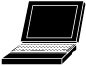
\includegraphics[scale=\ciscoImageScale]{\cisco/laptop}};

\draw[-] (Router)--node[yshift=0.5cm]{Old Connection}(Victim);
\draw[red, very thick] (Router)--node{New Connection}(Attacker);
\draw[red, very thick] (Attacker)--node{New Connection}(Victim);


\end{tikzpicture} 
\end{center}


	\begin{figure}[h]
		\caption{Photo depicting a MITM attack}
	\end{figure}
\end{center}

\subsubsection{Custom Router - Raspberry Pi}
As mentioned previously the effects will be performed on a custom computer acting as the router, because the network will be set-up to pass all traffic through this router, it will be able to simulate degradation on the entire networks traffic.
The Raspberry Pi \citep{upton2014raspberry} has been decided as the choice for the small custom computer. Originally designed to teach children to code on an inexpensive (less than £30) computer, the Pi has now found itself involved in a multitude of uses ranging from NAS (Network Attached Server) to robot controllers. The Pi's versatility is useful in this project due to its ease to set-up as a router, this is because of the easy access of low level aspects of the operating system due to it running a Linux based OS. The Raspberry Pi will be run with its default Raspbian OS \citep{pi2014raspbian} that is built upon Debian \citep{murdock1994overview}. This is a optimised OS for the internal ARM CPU that allows the Raspberry Pi to run modern stripped down programs on its very limited hardware, where however, it will have plenty of power to easily handle traffic as a router.



\subsubsection{Router alternatives}

\subsubsection*{MinnowBoard}
MinnowBoard \footnote{\url{https://minnowboard.org/}} is a company specialising in open source custom made processing units designed to remain compact while still being able to perform relatively heavy computation. Even their basic options have more RAM and processing speeds compared to that of the Raspberry Pi, but this comes at a higher cost, the basic model retails in at £110, more than 3 times to price of the Raspberry Pi. The increased processing speed would mean the total bandwidth capacity of the router could increase and would even allow the use of the GUI as an alternative to the command line, but this extra cost and increased processing speed does not add any extra value to the goal of the project and therefore the option was discarded.

\subsubsection*{Commercial router}
A commercial out-of-the-box router could be used with a custom version of OpenWrt \footnote{\url{https://openwrt.org/}}. OpenWrt is a custom version of Linux that is designed for embedded devices. To install this version of Linux on a router would require `flashing' the software. Flashing is the process of overwriting the embedded EEPROM or other type of embedded memory with the firmware of your choice, this process is lengthy and has no guarantee of working. This process however would provide the project with a device that could run the degradation script that is fully designed to function within a network, this could possibly mean faster processing speeds and a smoother experience. However, due to the uncertain set-up time compared to that of the Raspberry Pi this option was decided against. However, the option could be an aspect to implement in the long term improvements, this will be further discussed later in the report.

%<---- Checking done to here

%Comparison of Technologies:
%If there are several possible technologies that could be used in your project work you should present a comparative analysis and critical appraisal of each of these technologies. You should create a subsection for each of the technologies you discuss and title each subsection with the name of the technology it describes (e.g. object-oriented databases, XML ). Within each subsection you should provide an overview of the technology, its key features and its strengths and weaknesses in relation to your project.
\clearpage
\section{Comparison of Technologies}
\subsection{Protocol Comparison}
\subsubsection{TCP Based Protocols}

\subsubsection*{HTTP}
TCP has various protocols built on top of it. One of the most widely used protocols is HTTP/1.1 \citep{HTTP}. HTTP is a structured language used to transfer data worldwide. HTTP's main use is the movement of web based data, this has been chosen as one of the protocols to be used in the test network to simulate live traffic. Its use is due to the protocols heavy use in the real world. HTTP will be utilised by a web browser that attempts to access a web page, the degradation will therefore be visible through how quickly the web page loads and how responsive the connection seems.

\subsubsection*{FTP}
Another protocol based on top of TCP is FTP (File Transfer Protocol) \citep{FTP}, and as the broken down acronym suggests, this protocol is used to transfer files across a network. FTP has been selected also due to its integral use in a live network. It also has a quite intuitive way of representing the speed of a network through a download speed that is easy to understand for most users. The protocol will be tested with dummy files ranging from 1MB to 5GB. This size range was chosen to fully cover the normal spectrum of file size where it roughly ranges from a Word document to a high quality video.

\subsubsection*{Other TCP Considerations}

\subsubsection*{SFTP}
SFTP (SSH File Transfer Protocol) \citep{SFTP} was a consideration as a protocol to be used for the demonstration purposes. SFTP effectively is a secure version of FTP (but not to be mixed up with the Simple File Transfer Protocol). This was decided not to be used because of its added features such as authentication does not fit within the scope of the project, and does not relate to network degradation. 

\subsubsection*{Mail based protocols}
Another widely used set of protocols are the email based family of protocols. SMTP (Simple Mail Transfer Protocol) is involved in the sending of mail, while examples like IMAP/POP are used for receiving mail. These protocols use TCP as their transport layer protocols and are fundamental to email functioning on the internet, however, visualisation into their degradation would be no different to that of bare TCP. The implementation of an email client therefore, would add unnecessary complexity while offering almost zero added value to the demonstrative purposes of this project.


\subsubsection{UDP Based Protocols}
\begin{wrapfigure}{R}{5cm}
\begin{center}
	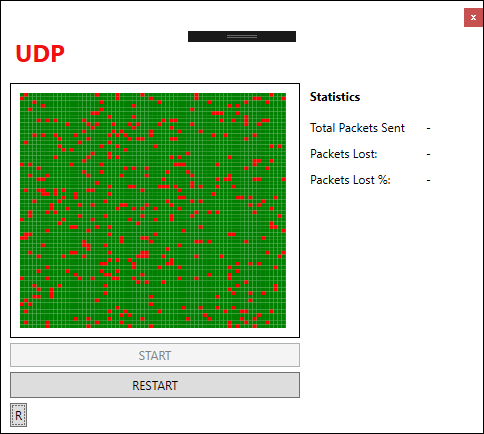
\includegraphics[scale=0.4]{UDP-Demo}
	\caption{Initial draft of the UDP user interface}
\end{center}
\end{wrapfigure}

UDP is hugely affected by packet loss due to its inherent unreliability. The effects on UDP have decided to be visualised by a program that simulates image transfer by assigning an individual UDP packet a number that corresponds to a single pixel, this packet is then sent. Once the server receives the packet, it reads the pixel number stored in the packet and changes that specific pixel to green. This creates a matrix of red (lost) and green (received) pixels. This therefore, gives a simple but effective visualisation of packet loss. 

Other effects can also be performed on UDP to simulate degradation. Latency and the incorrect arrival order of the packets are big signs of hostile transfer conditions and therefore, monitoring of the latency and order can be performed by the interface and could provide a much more detailed overview of the current health of the connection.

\subsubsection*{Other UDP based protocols}
UDP is used for situations where speed is required but reliability is not. Media streaming is a common example, lots of data needs to arrive to the client quickly where a small number of missed segments can go unnoticed. However, this kind of implementation would be a huge overhead. Even if 3rd party application was used it would not provide much more insight into what is happening to the protocol when the degradation is active. This is why UDP had been left as bare boned as possible and the protocol has been left relatively exposed to allow an effective way to visualise the effects.

\subsubsection{Other protocols}
\subsubsection*{QUIC}
Quick UDP Internet Connections \citep{hamilton2016quic} is an early stage transport layer protocol developed by Google where it was announced in 2013. QUIC is built upon UDP and is designed to provide faster transfer speed in web applications that utilise TCP.
It has a multitude of extra features, involving bandwidth estimation to reduce congestion, movement of congestion control into the application space rather than having the control embedded into the kernel meaning applications can adapt quicker and provide more bespoke decisions. QUIC also attempts to reduce latency by the simple inclusion of performing less transfers from that of an equivalent TCP connection. QUIC also includes techniques to attempt the handling of packet loss better than that of TCP. Techniques like: proactive speculative retransmissions ('Important' data is sent more than once).

There were initially concerns about UDP connectivity and the possibility that many users would be behind systems that block UDP traffic. This was mitigated by Chromium connectivity experiments \citep{roskind2013quic} where 91-94\% of Google users could make a UDP connection outbound.

QUIC was not chosen as an addition to this project due to it being in its infancy, where its adoption is still within the early stages. There are however, available open source client and server pairs available and the inclusion of this transport protocol would be a good addition in potential future work.

\subsubsection*{SPDY}
SPDY \citep{belshe2012spdy} is a Google created transport protocol designed to transfer web content. Its name is not an acronym and is pronounced "Speedy". SPDY works by manipulating HTTP traffic with the goals of reducing web load, latency and improving web security. However, in 2015 the protocol was deprecated by Google \citep{blog2015hello}, this was mainly due to the timing of the release of HTTP/2 where the improvements of SPDY were present in the upcoming version of HTTP. Full support for SPDY was removed in 2016. Due to SPDYs depreciation it was discarded as an option for this project.

\subsection{Operating Systems}

\subsubsection{Linux}
Linux is the broad definition of a family of computer operating systems. The defining characteristics of a ``Linux" OS is the free and open source approach and the use of the Linux Kernel. Android, for example, has the largest market share in the mobile OS market \citep{share2015desktop}, Android utilises the Linux kernel as the centre for its operating system.

Linux was chosen for this project for its open source element that allows easy access to low-level features in the kernel. The section of the kernel that deals with the filtration of packets for uses like firewalls and packet sniffers is referred to as the ``NetFilter". This acts as an API of sorts where packets can be routed to the net-filter queue to await a verdict (accept or drop) before being moved on. This is the basis for the functionality of the program. The program will run on the Raspberry Pi and route all packets that enter the box to the queue where the effects can be applied.


\subsubsection{Windows}
\label{ref:Windows}
Linux was chosen over the other possible alternative; Windows. The Windows OS is distributed as closed source software under proprietary licences meaning to understand what is happening under the hood is far more difficult. Windows does provide a solution to the packet filtering in the same way that NetFilter does, it is called Windows Filtering Platform (WFP) and it is a an API that allows access to the systems services in order to create packet filtering applications.

Windows, however, was not used because of the size of the Windows OS. Figure~\ref{ref:windowsRequire} contains the minimum system requirements for Windows 10 \footnote{\url{https://www.microsoft.com/en-US/windows/windows-10-specifications}}

%Windows Min System Requirements Table

\vspace{5mm} 
\begin{center}
\begin{tabular}{| l | l |}
	\hline
	Processor & 1 gigahertz (GHz) or faster processor or SoC \\
	RAM & 1 gigabyte (GB) for 32-bit or 2 GB for 64-bit \\
	Hard Disk Space & 16 GB for 32-bit OS 20 GB for 64-bit OS \\
	\hline
\end{tabular}
\begin{figure}[h]
		\caption{Windows System Requirements}
	\label{ref:windowsRequire}
	\end{figure}
\end{center}

\begin{wrapfigure}{r}{5cm}
\begin{center}
No Desktop\\
\begin{tabular}{| l | l |}
	\hline
	Processor & 1GHZ Pentium 4 \\
	RAM & 128 MB \\
	Hard Disk Space & 2 GB \\
	\hline
\end{tabular}

\vspace{2.5mm}

With Desktop\\
\begin{tabular}{| l | l |}
	\hline
	Processor & 1GHZ Pentium 4 \\
	RAM & 512 MB \\
	Hard Disk Space & 10 GB \\
	\hline
\end{tabular}
\caption{Debian system requirements}
\label{ref:debianRequire}
\end{center}
\end{wrapfigure}

This compared with the full Debian \footnote{\url{https://www.debian.org/releases/stable/i386/ch03s04.html.en}} OS that the stripped down version of the Raspberry Pi's OS is based off:

The Raspberry Pi in this instance will be run with no desktop.

As you can see from Figure~\ref{ref:debianRequire} the Linux based OS has a much smaller set of requirements. RAM usage for example, is 8 times smaller. Therefore, due to Linux's transparency and overall efficiency the OS is far more suited for use in conjunction with the Raspberry Pi. 

\clearpage
%Alternative Solutions:
%If others have produced solutions or addressed similar problems to those addressed by your project you should describe those alternative solutions here. Similarly, if several possible approaches suggest themselves as ways of solving the problems inherent in your project you should discuss those here. You should provide a comparative analysis and critical appraisal of each alternative solution approach or existing solution, identifying their key features and their strengths and weaknesses in relation to your project.
\section{Alternative Solutions}
\subsection{clumsy}
A more modern application of network degradation is clumsy 0.2 \footnote{\url{http://jagt.github.io/clumsy/index.html}}. It provides various options (that can run in parallel) that affect network conditions. 

\begin{wrapfigure}{r}{5cm}
\begin{center}
	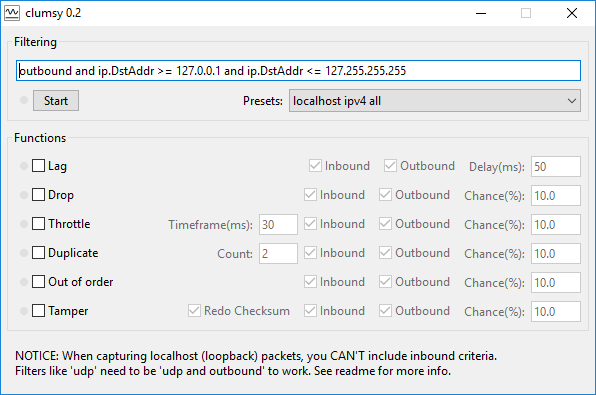
\includegraphics[scale=0.3]{clumsy}
	\caption{UI of clumsy}
\end{center}
\end{wrapfigure}

The tool provides a way to affect network conditions. It solves issues involved with simulating harsh network conditions. It does allow for filtering and has a couple of filter pre-sets, it however, does not provide options to simulate live traffic and controls to capture or visualise traffic is not part of the main package.

This tool provides and easy to use and simple tool that requires no extra download and can be run straight from the .exe, however, this only works on Windows machines and it uses the WFP API that was mentioned in Section~\ref{ref:Windows}. It also only affects the traffic on the local machine, this is good for testing tools in the development stage of an application but cannot easily be used to simulate degradation across a live network.

\subsection{TMNetSim}
TMNetSim \footnote{\url{http://www.tmurgent.com/appv/en/87-tools/performance-tools/177-tmnetsim-quick-and-easy-network-simulation-tool}} is another tool that covers aspects of this project. Unlike clumsy, TMNetSim is designed to provide degradation that expands over the network. However, to achieve this it has to be set-up on every machine, this is clunky and time consuming. The degradation script can negate this lengthy set-up with the intended inclusion of the ARP Spoofing (See Section~\ref{ref:arpSpoof})that will allow rapid deployment of the script between target and router. There is further criticism relating to the ease of use of this application, it has a large number of controls on its interface and will involve a larger learning curve to master compared to other simpler tools, this however might be the bi-product of more functionality; increased complexity.

This tool includes very complex ways of simulating realistic degradation with ``Gaussian" and ``Normal" delay modes, that attempt to provide more accurate representations of real-world delays. This is a great feature that could drastically improve the accuracy in simulating degradation and will need to be considered as an extra inclusion into this project.

\subsection{Comcast}
Comcast \footnote{\url{https://github.com/tylertreat/comcast}} is a tool designed to test systems in non-critical ways. It is only a thin wrapper around tools such as `iptables`, `tc', `ipfw' and `pfctl'. It makes it very easy to add latency, packet loss and error to a data stream. The script is written in Go and runs terminal instances for each command.

The script allows very basic degradation to be performed but, because it is strongly coupled to other tools it means it is not very dynamic and new effects cannot be quickly added to the program.

This solution is very useful in applying quick and easy degradation to a single client but because of its lack off malleability the tool would be hard to apply to many situations.